\documentclass[tikz,border=2pt]{standalone}
\usepackage{amsmath}
\usepackage{pgfplots}
\pgfplotsset{compat=1.18}

\begin{document}
% f(x)=x^3/3-x, its derivative f'(x)=x^2-1 and second derivative f''(x)=2x: each derivative
% describes the slope of the one before it.
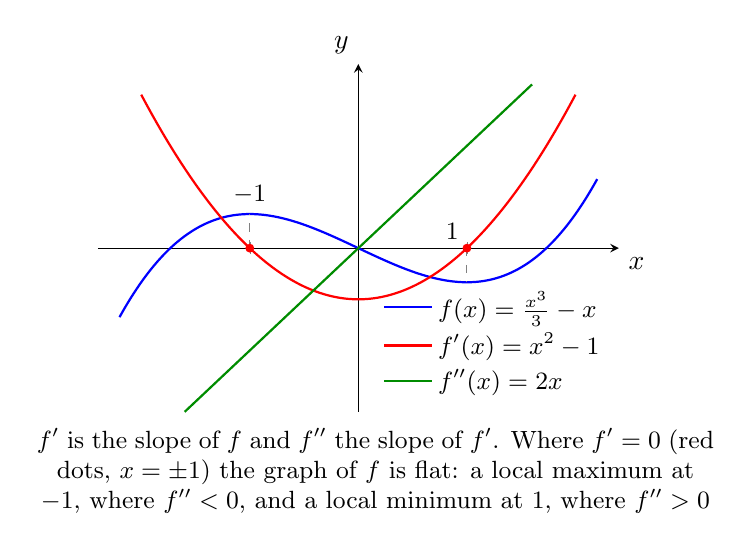
\begin{tikzpicture}
	\begin{axis}[
		axis lines=middle,
		xmin=-2.4, xmax=2.4,
		ymin=-3.2, ymax=3.6,
		xtick={-1,1}, xticklabels={,}, ytick=\empty,
		xlabel={$x$}, ylabel={$y$},
		xlabel style={below right}, ylabel style={above left},
		samples=140, smooth, clip=false,
		width=8.2cm, height=6cm,
		legend style={at={(0.99,0.02)}, anchor=south east, draw=none, fill=none, font=\small}, legend cell align=left
		]
		\addplot[thick, blue, domain=-2.2:2.2] {x^3/3-x};
		\addlegendentry{$f(x)=\tfrac{x^3}{3}-x$}
		\addplot[thick, red, domain=-2.0:2.0] {x^2-1};
		\addlegendentry{$f'(x)=x^2-1$}
		\addplot[thick, green!55!black, domain=-1.6:1.6] {2*x};
		\addlegendentry{$f''(x)=2x$}
		\draw[dashed, gray] (axis cs:1,0) -- (axis cs:1,-0.667);
		\draw[dashed, gray] (axis cs:-1,0) -- (axis cs:-1,0.667);
		\node[anchor=south east, font=\small, inner sep=2pt] at (axis cs:0.98,0.05) {$1$};
		\node[anchor=south, font=\small, inner sep=2pt] at (axis cs:-1,0.75) {$-1$};
		\fill[red] (axis cs:1,0) circle (1.6pt);
		\fill[red] (axis cs:-1,0) circle (1.6pt);
	\end{axis}
	\node[anchor=north, font=\small, align=flush center, text width=8.6cm] at ([yshift=-2pt]current axis.outer south) {$f'$ is the slope of $f$ and $f''$ the slope of $f'$. Where $f'=0$ (red dots, $x=\pm1$) the graph of $f$ is flat: a local maximum at $-1$, where $f''<0$, and a local minimum at $1$, where $f''>0$};
\end{tikzpicture}
\end{document}
